\subsection{Semantics}\label{subsec:semantics}
\begin{comment}
Where do most of our semantics come from?

Intersection semantics
- Motivation

Describe union semantics
- Motivation
- New definition
- Visual change

Describe MatchAny semantics
- Motivation
- Definition
- Visual
\end{comment}

Most of the semantics on constructing TAs from TREs have been copied directly from the paper by Asarin et al. \cite{Eugene2001}. However, we have made modifications to some of the semantics described in the paper.

\subsubsection{Intersection}
When creating TAs using an intersection with the rules from Asarin et al.
many states are created with no transitions.
By creating the intersection states lazily as needed for transitions, we can greatly decrease the number of states created.

\subsubsection{Union}
The epsilon transitions from the union semantics of Asarin et al. can be slightly optimized, by only creating an extra epsilon transition when there is a loop going back to the initial state.
An updated version of the union semantics can be seen in \cref{def:union-semantics}.

% We can improve upon union by removing unnecessary epsilon transitions.
\begin{definition}
    Union\label{def:union-semantics}
    
    \sembox{
        $\semaut{\varphi_1|\varphi_2}=
        \left\{\begin{array}{ll}
            \semaut{(\epsilon\cdot\varphi_1)\cup\varphi_2} & if (q_1,\phi_1,p_1,a,s_1)\in\Delta_1 \\
            \semaut{\varphi_1\cup(\epsilon\cdot\varphi_2)} & if (q_2,\phi_2,p_2,a,s_2)\in\Delta_2 \\
            \automaton & otherwise \\
        \end{array}\right.
        $
        
        Where
        
        $f\transition=
        \left\{\begin{array}{ll}
            \transition[][s] & if q\in\{s_1,s_2\} \\
            \transition & otherwise \\
        \end{array}\right.
        $
        
        $Q=Q_1\cup Q_2 \cup {s}\backslash\{s_1,s_2\}$
        
        $C=C_1\cup C_2$
        
        $\Delta=f(\Delta_1\cup\Delta_2)$
        
        $F=F_1\cup F_2\backslash\{s_1,s_2\}$
    }
\end{definition}

The semantics work by checking if there is a transition looping back to the initial state on either TAs.
If this is the case, they are concatenated with an epsilon TRE.
That means in the case where both TAs have a transition to their initial state, our new semantics will create the same result as the one in the paper.
However, when a TA does not have a transition back to the initial state, we do not need the extra epsilon transition, as the purpose of the extra transition is to make sure you can not first take a loop in one TA, and then move to the other TA. An example of this rule can be seen on \cref{fig:union}.

% We can improve upon union by removing unnecessary epsilon transitions.
\begin{definition}
    Union\label{def:union-semantics}
    
    \sembox{
        $\semaut{\varphi_1|\varphi_2}=
        \left\{\begin{array}{ll}
            \semaut{(\epsilon\cdot\varphi_1)\cup\varphi_2} & if (q_1,\phi_1,p_1,a,s_1)\in\Delta_1 \\
            \semaut{\varphi_1\cup(\epsilon\cdot\varphi_2)} & if (q_2,\phi_2,p_2,a,s_2)\in\Delta_2 \\
            \automaton & otherwise \\
        \end{array}\right.
        $
        
        Where
        
        $f\transition=
        \left\{\begin{array}{ll}
            \transition[][s] & if q\in\{s_1,s_2\} \\
            \transition & otherwise \\
        \end{array}\right.
        $
        
        $Q=Q_1\cup Q_2 \cup {s}\backslash\{s_1,s_2\}$
        
        $C=C_1\cup C_2$
        
        $\Delta=f(\Delta_1\cup\Delta_2)$
        
        $F=F_1\cup F_2\backslash\{s_1,s_2\}$
    }
\end{definition}
\captionof{figure}{Example of union semantics on: $A|B$ (TOP) and $A+|B$ (BOTTOM).}
\label{fig:union}
\vspace{1em}

These new union semantics are not entirely equivalent to the ones described by Asarin et al., since we removed the time constraint from the epsilon edges.
This time constraint creates an error that makes the TRE and the TA accept different languages.
This mistake, and what we did to fix it, is further described in \cref{sec:PaperCorrections}

\subsubsection{Match any}
Only match on a single character was defined in the paper by Asarin et al. and we wanted to have a way to match all possible characters like normal regular expressions. For this we used a '.' like in normal regular expressions. Transitions with this symbol are allowed to be taken like any other transition when any input is given. Otherwise, this symbol is the same as all other symbols in the TA.

\usetikzlibrary {automata,positioning}
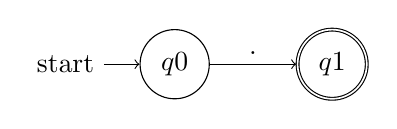
\begin{tikzpicture}[auto]
    \node[state, initial] at (0, 0)(q0){$q0$};
    \node[state, accepting] at (2, 0)(q1){$q1$};
    
    \path[->]
        (q0)edge node{$.$}(q1)
        ;
\end{tikzpicture}

